%Correct the file name.
%X: book number
%Y: part number
%ZZZ: page number in three digits. So page 3 would be 003.

\documentclass[11pt]{amsbook}

\usepackage{../HBSuerDemir}	% ------------------------


\begin{document}

% ++++++++++++++++++++++++++++++++++++++
\hPage{b1p2/249}
% ++++++++++++++++++++++++++++++++++++++
	\begin{enumerate}
		\item[11.]
		Same question for :
		\[ \left|
	     \begin{array}{cccc}
	        0 & a & b & c\\
	        a & 0 & c & b\\
	        b & c & 0 & a\\
	        c & b & a & 0
		\end{array}
    	\right| \]

    	\item[12.]
    	Prove the equality :
    	\[ \left| \begin{array}{llll}
	        0 & a^2 & b^2 & c^2\\
	        a^2 & 0 & f^2 & e^2\\  
	        b^2 & f^2 & 0 & d^2\\
	        c^2 & e^2 & d^2 & 0
    	\end{array} \right|
    	=
    	\left| \begin{array}{cccc}
	        0 & 1 & 1 & 1\\
	        1 & 0 & c^2f^2 & b^2e^2\\
	        1 & c^2f^2 & 0 & a^2d^2\\
	        1 & b^2c^2 & a^2d^2 & 0
    	\end{array} \right| \] 

    	\item[13.]
    	Prove
    	\[ \left| \begin{array}{llll}
	        0 & 1 & 1 & 1\\
	        1 & 0 & c^2 & b^2\\  
	        1 & c^2 & 0 & a^2\\
	        1 & b^2 & a^2 & 0
	    \end{array} \right|
	    =
	    \left| \begin{array}{cccc}
	        0 & a & b & c\\
	        a & 0 & c & b\\  
	        b & c & 0 & a\\
	        c & b & a & 0
    	\end{array} \right|
    	=
    	-16\Delta^2,
		\]
    	
		\item[14.]
		If
		\[ \left| \begin{array}{cccc}
	        1 & a & a^2 & a^3\\
	        1 & b & b^2 & b^3\\  
	        1 & c^2 & 0 & a^2\\
	        1 & b^2 & a^2 & 0
   		 \end{array} \right|
    		=
    		0 
    	\] 
     	show that at least two of the numbers a, b, c, d must be equal to each other.

    	\item[15.]
    	Show that the determinant
    	$\begin{vmatrix}
		a_{ij} & + & x 
		\end{vmatrix}$
		of order n is of the form E + Fx where E, F are independent of x.

		\item[16.]
		Show that one root of the equation
	\end{enumerate}
\end{document}  

%==== templates ====

%==== environments ====

%\begin{figure}[htb]
%	\centering
%	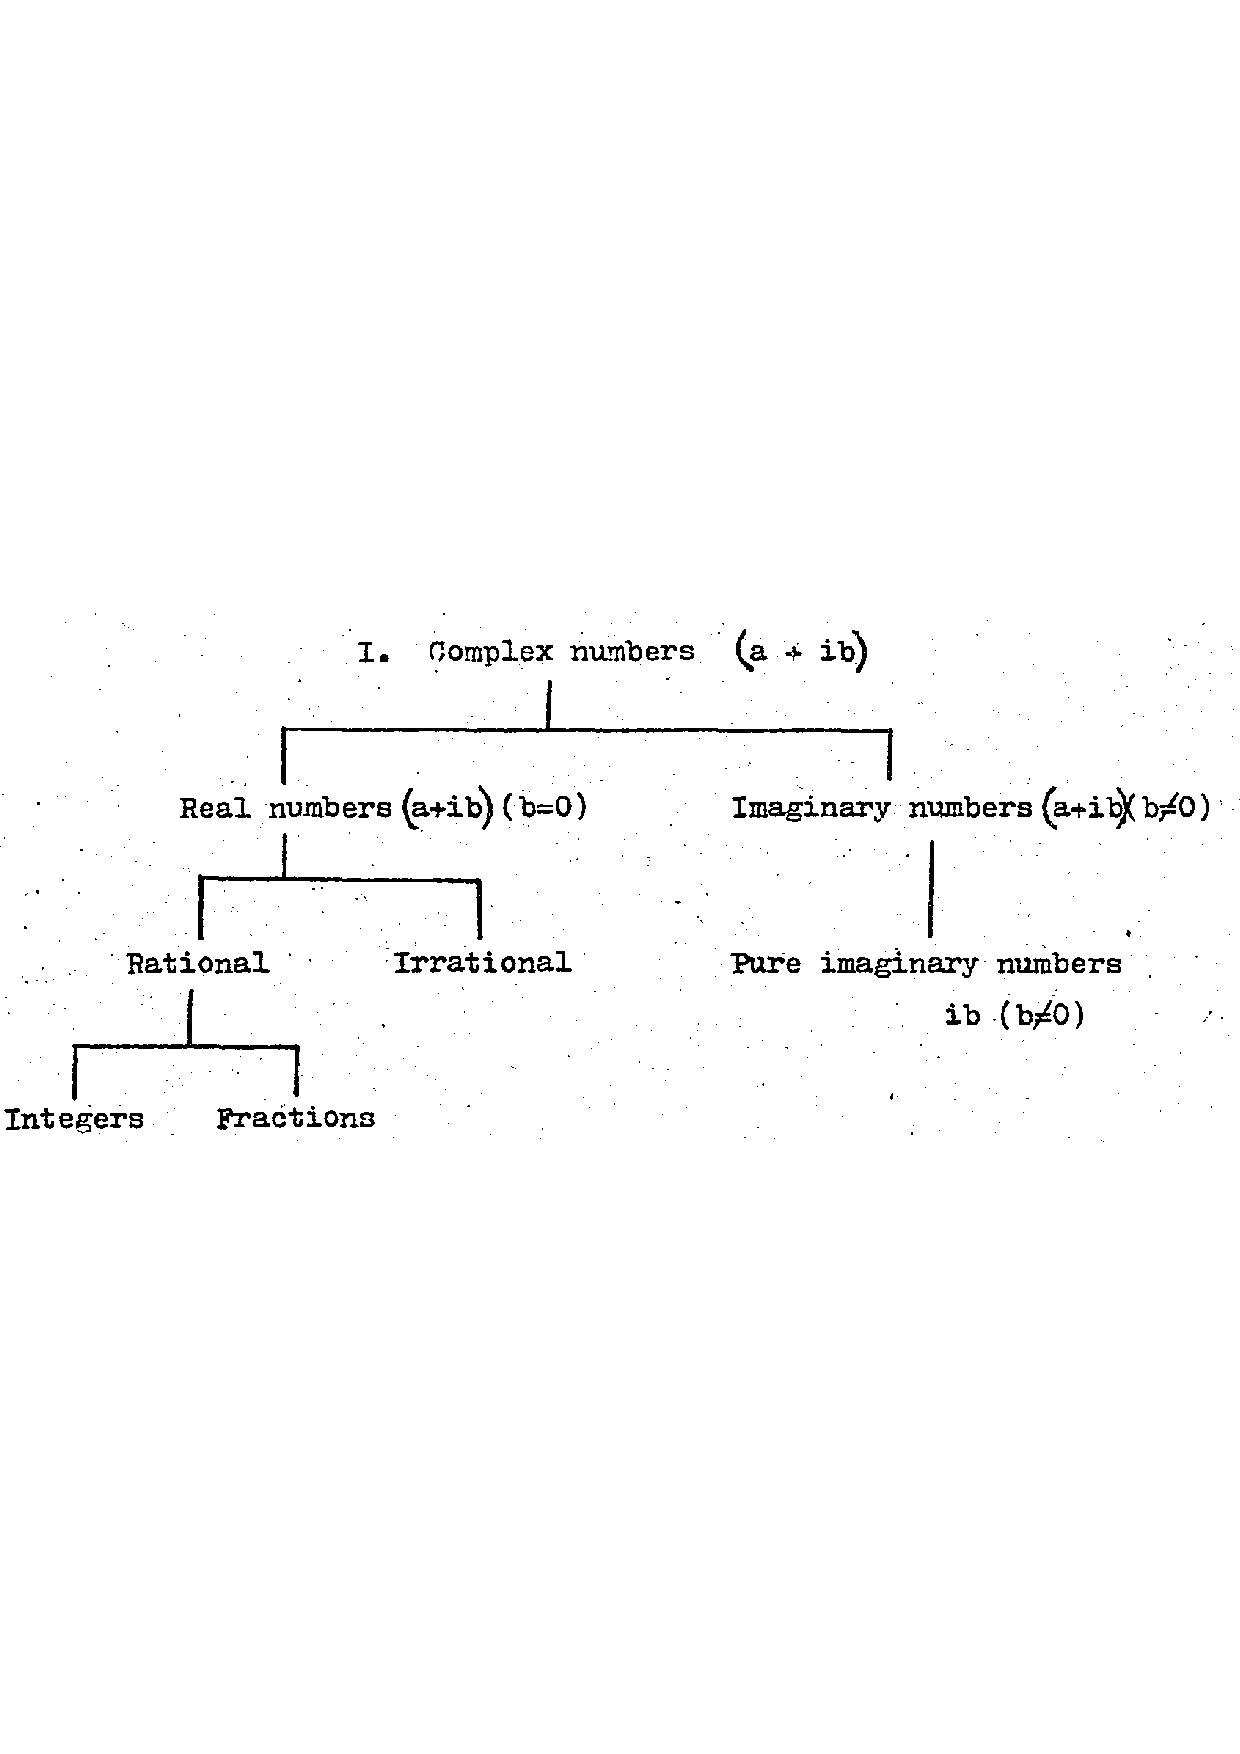
\includegraphics[width=0.9\textwidth]{images/SD-1-1p15A}
%	\caption{Classification of complex numbers}
%	\label{fig:classificationOfComplexNumbersA}
%\end{figure}

%\begin{center}
%\begin{tabular}{cc}
%\end{tabular}
%\end{center}

%\begin{exmp}
%\begin{hSolution}
%\end{hSolution}
%\end{exmp}

%\begin{hEnumerateAlpha}
%\end{hEnumerateAlpha}

%\begin{hEnumerateRoman}
%\end{hEnumerateRoman}

%$
%\begin{bmatrix}
%\end{bmatrix}
%$

%\frac{aaaa}{bbb}
%\frac{a_{n}}{b_{n}}
%\left( aaaa \right)
%\Longrightarrow

%\begin{multicols}{2}
%	bb
%\columnbreak
%	aa
%\end{multicols}
